\subsection{Upper integral of a positive function}

For every numerical function \(f \geqslant 0\) (finite or not) defined on X, there exist functions \(h \in J_{+}\) such that \(f \leqslant h\) , if none other then the constant \(+\infty\) .

DEFINITION 3. --- Let \(\mu\) be a positive measure on X; for every numerical function \(f \geqslant 0\) (finite or not) defined on X, the positive number

\[
\mu^ {*} (f) = \inf _ {h \geqslant f, h \in \mathscr {I} _ {+}} \mu^ {*} (h)
\]

(finite or equal to \(+\infty\) ) is called the upper integral of \(f\) (with respect to \(\mu\) ).

When \(f \in \mathcal{I}_+\) , the number \(\mu^*(f)\) thus defined is equal to the upper integral defined in Def. 1, since \(\mu^*\) is increasing in \(\mathcal{I}_+\) .

In place of the notation \(\mu^{*}(f)\) , we shall also employ the notations \(\int^{*} f d\mu\) , \(\int^{*} f(x) d\mu(x)\) , \(\int^{*} f\mu\) and \(\int^{*} f(x)\mu(x)\) .

Example. --- If X is a discrete space, \(\mu\) a positive measure on X, and if one sets \(\alpha(x) = \mu(\varphi_{\{x\}})\) , then \(\mu^{*}(f) = \sum_{x \in X} \alpha(x)f(x)\) for every numerical function

\(f \geqslant 0\) defined on X, since such a function is continuous (No.~1, Example).

PROPOSITION 10. --- If \(f\) and \(g\) are two numerical functions \(\geqslant 0\) defined on \(X\) such that \(f \leqslant g\) , then \(\mu^{*}(f) \leqslant \mu^{*}(g)\) .

PROPOSITION 11. --- For every finite real number \(\alpha > 0\) and every numerical function \(f \geqslant 0\) defined on X,

\[
\mu^ {*} (\alpha f) = \alpha \mu^ {*} (f).\tag{8}
\]

PROPOSITION 12. --- If \(f_1\) and \(f_2\) are two numerical functions \(\geqslant 0\) defined on \(X\) , then

\[
\mu^ {*} (f _ {1} + f _ {2}) \leqslant \mu^ {*} (f _ {1}) + \mu^ {*} (f _ {2}).\tag{9}
\]

For every function \(h_1 \in \mathcal{I}_+\) such that \(f_1 \leqslant h_1\) and every function \(h_2 \in \mathcal{I}_+\) such that \(f_2 \leqslant h_2\) , we have, by Th. 2,

\[
\mu^ {*} (f _ {1} + f _ {2}) \leqslant \mu^ {*} (h _ {1} + h _ {2}) = \mu^ {*} (h _ {1}) + \mu^ {*} (h _ {2}),
\]

whence (GT, IV, §5, No.~7, Cor. 2 of Prop. 12)

\[
\mu^ {*} (f _ {1} + f _ {2}) \leqslant \inf _ {h _ {1} \geqslant f _ {1}, h _ {1} \in \mathcal {I} _ {+}} \mu^ {*} (h _ {1}) + \inf _ {h _ {2} \geqslant f _ {2}, h _ {2} \in \mathcal {I} _ {+}} \mu^ {*} (h _ {2}),
\]

which is none other than the inequality (9).

Props. 10, 11 and 12 express that \(\mu^{*}\) is an increasing, positively homogeneous and convex function on the set of numerical functions \(\geqslant 0\) defined on X (Ch. I, No.~1). Note that if \(f_{1}\) and \(f_{2}\) are any two positive functions, the two members of (9) are not necessarily equal ( \(\S 4\) , Exer. 8 \(d\) ); in \(\S 5\) , No.~6 we shall give conditions under which equality holds.

THEOREM 3. --- For every increasing sequence \((f_{n})\) of numerical functions \(\geqslant 0\) defined on X,

\[
\mu^ {*} \left(\sup _ {n} f _ {n}\right) = \sup _ {n} \mu^ {*} (f _ {n}).\tag{10}
\]

Since each of the functions \(f_n\) is less than or equal to \(\sup_{n} f_n\) , everything comes down to proving that \(\mu^*(\sup_{n} f_n) \leqslant \sup_{n} \mu^*(f_n)\) ; this is obvious if the second member of the inequality is \(+\infty\) . In the contrary case, \(\mu^*(f_n) < +\infty\) for all \(n\) ; we are going to show that, for every \(\varepsilon > 0\) , there exists an increasing sequence \((g_n)\) of functions in \(\mathcal{I}_+\) such that \(f_n \leqslant g_n\) and \(\mu^*(g_n) \leqslant \mu^*(f_n) + \varepsilon\) . If \(g\) is the upper envelope of the sequence \((g_n)\) , we will then have \(\mu^*(g) = \sup_n \mu^*(g_n)\) (No.~1, Th. 1), whence \(\mu^*(g) \leqslant \sup \mu^*(f_n) + \varepsilon\) ; since \(\sup f_n \leqslant g\) and \(\varepsilon\) is arbitrary, the theorem will then have been proved.

By hypothesis, there exists a function \(h_{n} \in I_{+}\) such that \(f_{n} \leqslant h_{n}\) and \(\mu^{*}(f_{n}) \leqslant \mu^{*}(h_{n}) \leqslant \mu^{*}(f_{n}) + \varepsilon/2^{n}\) ; let us show that the functions \(g_{n} = \sup(h_{1}, h_{2}, \ldots, h_{n})\) meet the requirements. They belong to \(I_{+}\) , form an increasing sequence, and satisfy \(f_{n} \leqslant g_{n}\) for all n; we shall prove that

\[
\mu^ {*} (g _ {n}) \leqslant \mu^ {*} (f _ {n}) + \varepsilon \left(1 - \frac {1}{2 ^ {n}}\right).
\]

Let us argue by induction on \(n\) ; the case \(n = 1\) is trivial. On the other hand \(g_{n+1} = \sup(g_n, h_{n+1})\) , \(g_n \geqslant f_n\) and \(h_{n+1} \geqslant f_{n+1} \geqslant f_n\) , whence \(\inf(g_n, h_{n+1}) \geqslant f_n\) ; since

\[
\inf (g _ {n}, h _ {n + 1}) + \sup (g _ {n}, h _ {n + 1}) = g _ {n} + h _ {n + 1},
\]

it follows from Th. 2 of No.~1 that

\[
\begin{array}{l} \mu^ {*} (g _ {n + 1}) = \mu^ {*} (g _ {n}) + \mu^ {*} (h _ {n + 1}) - \mu^ {*} \big (\inf (g _ {n}, h _ {n + 1}) \big) \\ \leqslant \mu^ {*} (g _ {n}) + \mu^ {*} (h _ {n + 1}) - \mu^ {*} (f _ {n}) \\ \leqslant \mu^ {*} (f _ {n + 1}) + \varepsilon \left(1 - \frac {1}{2 ^ {n}}\right) + \frac {\varepsilon}{2 ^ {n + 1}} \\ = \mu^ {*} (f _ {n + 1}) + \varepsilon \left(1 - \frac {1}{2 ^ {n + 1}}\right). \end{array}\tag{Q.E.D.}
\]

COROLLARY. --- Let F be a set of numerical functions \(\geqslant 0\) , directed for the relation \(\leqslant\) , such that there exists a countable cofinal subset G of F (S, III, §1, No.~7); then

\[
\mu^ {*} \left(\sup _ {f \in \mathfrak {F}} f\right) = \sup _ {f \in \mathfrak {F}} \mu^ {*} (f).\tag{11}
\]

For, there exists an increasing sequence of functions in \(\mathfrak{G}\) having the same upper envelope as \(\mathfrak{F}\) : if \((f_n)\) is the sequence of functions of \(\mathfrak{G}\) , arranged in any order, let \((f_{n_k})\) be a subsequence defined recursively by the conditions \(n_1 = 1\) , \(f_{n_{k+1}} \geqslant \sup(f_{n_k}, f_k)\) ; it is clear that this subsequence has the indicated properties.

\pandocbounded{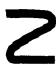
\includegraphics[keepaspectratio]{images/part001_ffa48347.jpg}}

Remarks. - 1) The relation (11) does not necessarily hold when \(\mathfrak{F}\) is an uncountable directed set of functions \(\geqslant 0\) that are not lower semi-continuous. Take for example \(X = R\) , \(\mu\) being Lebesgue measure on \(R\) , and consider the directed (for \(\leqslant\) ) set \(\mathfrak{F}\) of characteristic functions \(\varphi_{M}\) of all the finite subsets \(M\) of \(R\) . Then \(\mu^{*}(\varphi_{M}) = 0\) for every finite subset \(M\) , because a point is contained in an open interval of arbitrarily small length, and the characteristic function of a set reduced to a point therefore has upper integral zero by Def. 3 and Prop. 9 of No.~2. But the upper envelope of \(\mathfrak{F}\) is the constant function equal to 1, and \(\mu^{*}(1) = +\infty\) .

\begin{enumerate}
\def\labelenumi{\arabic{enumi})}
\setcounter{enumi}{1}
\tightlist
\item
  Note that for a decreasing sequence \((f_n)\) of functions \(\geqslant 0\) , one does not necessarily have \(\mu^{*}(\inf_{n} f_n) = \inf_{n} \mu^{*}(f_n)\) , even if \(\mu^{*}(f_n) < +\infty\) for all \(n\) (cf.~§4, Exer. 8 c)).
\end{enumerate}

PROPOSITION 13. --- For every sequence \((f_n)\) of numerical functions \(\geqslant 0\) defined on \(X\) ,

\[
\mu^ {*} \left(\sum_ {n = 1} ^ {\infty} f _ {n}\right) \leqslant \sum_ {n = 1} ^ {\infty} \mu^ {*} (f _ {n}).\tag{12}
\]

It suffices to apply the relation (10) to the increasing sequence of functions \(g_{n} = \sum_{k=1}^{n} f_{k}\) while taking into account that, by (9),

\[
\mu^ {*} (g _ {n}) \leqslant \sum_ {k = 1} ^ {n} \mu^ {*} (f _ {k}).
\]

In §5, No.~6, we will give conditions under which the two members of (12) are equal.

PROPOSITION 14 (Fatou's lemma). --- For every sequence \((f_{n})\) of numerical functions \(\geqslant 0\) ,

\[
\mu^ {*} \left(\liminf _ {n \to \infty} f _ {n}\right) \leqslant \liminf _ {n \to \infty} \mu^ {*} (f _ {n})  .\tag{13}
\]

For every integer \(n\) , set \(g_{n} = \inf_{p\geqslant 0}f_{n + p}\) ; the sequence \((g_n)\) is increasing and \(\liminf_{n\to \infty}f_n = \sup_n g_n\) , whence, by (10),

\[
\mu^ {*} (\liminf _ {n \to \infty} f _ {n}) = \sup _ {n} \mu^ {*} (g _ {n});
\]

but since \(g_{n} \leqslant f_{n+p}\) for \(p \geqslant 0\) , we have \(\mu^{*}(g_{n}) \leqslant \mu^{*}(f_{n+p})\) , whence \(\mu^{*}(g_{n}) \leqslant \inf_{p \geqslant 0} \mu^{*}(f_{n+p})\) and finally

\[
\mu^ {*} \left(\operatorname * {l i m i n f} _ {n \to \infty} f _ {n}\right) \leqslant \sup _ {n} \left(\inf _ {p \geqslant 0} \mu^ {*} (f _ {n + p})\right) = \operatorname * {l i m i n f} _ {n \to \infty} \mu^ {*} (f _ {n}).
\]

COROLLARY. --- Let \((f_{n})\) be a sequence of numerical functions \(\geqslant0\) such that, for every \(x\in X\) , \(\lim_{n\to\infty}f_{n}(x)=+\infty\) . If \(\mu\) is not the zero measure, then \(\lim_{n\to\infty}\mu^{*}(f_{n})=+\infty\) .

If \(f_{0}\) is the constant function equal to \(+\infty\) , then \(f_{0}\) is the upper envelope of all the functions of \(K_{+}\) , and, since \(\mu \neq 0\) , we have \(\mu^{*}(f_{0}) > 0\) ; but since \(f_{0} = \alpha f_{0}\) for every \(\alpha > 0\) , necessarily \(\mu^{*}(f_{0}) = +\infty\) (Prop. 11). The inequality (13) then shows that \(\mu^{*}(f_{n})\) tends to \(+\infty\) with n.

PROPOSITION 15. --- For every scalar \(\alpha > 0\) and every pair of positive measures \(\mu, \nu\) on \(X\) ,

\[
(\alpha \mu) ^ {*} = \alpha \mu^ {*}\tag{14}
\]

\[
(\mu + \nu) ^ {*} = \mu^ {*} + \nu^ {*}\tag{15}
\]

Moreover, the relation \(\mu \leqslant \nu\) implies \(\mu^{*} \leqslant \nu^{*}\) .

Let us prove the relation (15). Set \(\lambda = \mu + \nu\) ; thus \(\lambda(f) = \mu(f) + \nu(f)\) for \(f \in \mathcal{K}_+\) ; for \(f \in \mathcal{I}_+\) , the value of \(\lambda^*(f)\) (resp. \(\mu^*(f), \nu^*(f)\) ) is the limit of \(\lambda(g)\) (resp. \(\mu(g), \nu(g)\) ) as \(g\) runs over the directed set (for \(\leqslant\) ) of all \(g \in \mathcal{K}_+\) such that \(g \leqslant f\) ; therefore \(\lambda^*(f) = \mu^*(f) + \nu^*(f)\) . Finally, if \(f\) is any function \(\geqslant 0\) defined on X, then \(\lambda^*(f)\) (resp. \(\mu^*(f), \nu^*(f)\) ) is the limit of \(\lambda^*(h)\) (resp. \(\mu^*(h), \nu^*(h)\) ) as \(h\) runs over the directed set (for \(\geqslant\) ) of all functions \(h \in \mathcal{I}_+\) such that \(h \geqslant f\) ; again, by passage to the limit, we therefore have \(\lambda^*(f) = \mu^*(f) + \nu^*(f)\) , which proves (15). The relation (14) is established similarly. Finally, if \(\mu \leqslant \nu\) one can write \(\nu = \mu + (\nu - \mu)\) , where \(\nu - \mu \geqslant 0\) , therefore \(\nu^* = \mu^* + (\nu - \mu)^*\) , which shows that \(\mu^* \leqslant \nu^*\) .

